\documentclass{beamer}
\usetheme{Warsaw}
\usefonttheme[onlymath]{serif}
\usepackage{ctex}
\usepackage{amsmath}

\title{Pre}
\institute{兰州大学物理科学与技术学院}
\date{\today}

\begin{document}
\songti
\maketitle
\footnotesize

\section{外差干涉}
\begin{frame}{外差干涉}
    \footnotesize
    
设探测器表面上两束光的复振幅分别为 $U_{\mathrm{M}}=A_{\mathrm{M}}\exp\left[\mathrm{i}\left(\omega_{\mathrm{M}}t+\phi_{\mathrm{M}} \right)  \right] $ 和 $U_{\mathrm{R}}=A_{\mathrm{R}}\exp\left[\mathrm{i}\left(\omega_{\mathrm{R}}t+\phi_{\mathrm{R}}\right)  \right] $。其中,下标 $\mathrm{M} $ 代表测量光,下标 $\mathrm{R} $ 代表参考光。

外差干涉得到的光强为:

$$
\begin{aligned}
I
&=|U_{\mathrm{M}}+U_{\mathrm{R}} |^2 \\
&=\left|A_{\mathrm{M}}\exp\left[\mathrm{i}\left(\omega_{\mathrm{M}}t+\phi_{\mathrm{M}} \right)  \right] + A_{\mathrm{R}}\exp\left[\mathrm{i}\left(\omega_{\mathrm{R}}t+\phi_{\mathrm{R}}\right)  \right] \right|^2 \\
&=A_{\mathrm{M}}^2 + A_{\mathrm{R}}^2 + 2A_{\mathrm{M}}A_{\mathrm{R}}\cos[(\omega_{\mathrm{M}} - \omega_{\mathrm{R}})t + (\phi_{\mathrm{M}}-\phi_{\mathrm{R}})]
\end{aligned}
$$

定义两个物理量:

$$
\omega_{\mathrm{het}}
:=\omega_{\mathrm{M}} - \omega_{\mathrm{R}},~~
\phi_{\mathrm{het}}
:=\phi_{\mathrm{M}} - \phi_{\mathrm{R}}
$$

则光强可以写为:

$$
I
=A_{\mathrm{M}}^2 + A_{\mathrm{R}}^2 + 2A_{\mathrm{M}}A_{\mathrm{R}}\cos(\omega_{\mathrm{het}}t+\phi_{\mathrm{het}})
$$

\end{frame}

\begin{frame}

光强正比于平均电磁能流密度,不妨认为光强对探测器表面 $S $ 的面积分就是探测器接收的功率 $P $ ,即:

$$
\begin{aligned}
P
&=\int I\mathrm{d}S \\
&=\int \bigg[ A_{\mathrm{M}}^2 + A_{\mathrm{R}}^2 + 2A_{\mathrm{M}}A_{\mathrm{R}}\cos(\omega_{\mathrm{het}}t+\phi_{\mathrm{het}}) \bigg] \mathrm{d}S \\
&=P_{\mathrm{M}} + P_{\mathrm{R}} + \int 2 A_{\mathrm{M}}A_{\mathrm{R}}\cos(\omega_{\mathrm{het}}t+\phi_{\mathrm{het}})\mathrm{d}S \\
&=P_{\mathrm{M}} + P_{\mathrm{R}} + \mathrm{Re} \left\{\int 2 A_{\mathrm{M}}A_{\mathrm{R}}\exp(\mathrm{i}\omega_{\mathrm{het}} t)\cdot\exp(\mathrm{i} \phi_{\mathrm{het}}) \mathrm{d}S \right\} \\
&=P_{\mathrm{M}} + P_{\mathrm{R}} + \mathrm{Re} \left\{2\exp(\mathrm{i} \omega_{\mathrm{het}}t) \int A_{\mathrm{M}}A_{\mathrm{R}} \exp(\mathrm{i} \phi_{\mathrm{het}}) \mathrm{d}S \right\} \\
&=P_{\mathrm{M}} + P_{\mathrm{R}} + \mathrm{Re}\left\{2\exp(\mathrm{i} \omega_{\mathrm{het}}t)\cdot A\exp(\mathrm{i\phi}) \right\},~A\exp(\mathrm{i}\phi):=\int A_{\mathrm{M}}A_{\mathrm{R}} \exp(\mathrm{i} \phi_{\mathrm{het}}) \mathrm{d}S \\
&=P_{\mathrm{M}} + P_{\mathrm{R}} + 2A\cos(\omega_{\mathrm{het}}t + \phi) \\
&=P_{\mathrm{M}} + P_{\mathrm{R}} + 2\sqrt{P_{\mathrm{M}}P_{\mathrm{R}}}|o|\cos(\omega_{\mathrm{het}}t+\arg\{o \}),~o:=\frac{A\exp(\mathrm{i}\phi)}{\sqrt{P_{\mathrm{M}}P_{\mathrm{R}}}}
\end{aligned}
$$

\end{frame}

\begin{frame}
    
    一般来说,$A_{\mathrm{M}},A_{\mathrm{R}},\phi_{\mathrm{het}}$ 都是探测器表面坐标的函数。

    若考虑外差干涉的两束光均为平面波且正入射的情况,则探测器接收的功率可简化为:

    $$
    \begin{aligned}
    P
    =P_{\mathrm{M}} + P_{\mathrm{R}} + 2\sqrt{P_{\mathrm{M}}P_{\mathrm{R}}}|o|\cos(\omega_{\mathrm{het}}t+\phi_{\mathrm{het}})
    \end{aligned}
    $$

    其中,
    
    $$
    \omega_{\mathrm{het}} = \omega_{\mathrm{M}}-\omega_{\mathrm{R}},~~
    \phi_{\mathrm{het}} = \phi_{\mathrm{M}}-\phi_{\mathrm{R}}
    $$

    $$
    P_{\mathrm{M}} = \int A_{\mathrm{M}}^2\mathrm{d}S,~~P_{\mathrm{R}}=\int A_{\mathrm{R}}^2 \mathrm{d}S 
    $$

    $$
    o = \frac{\int A_{\mathrm{M}}A_{\mathrm{R}} \exp(\mathrm{i} \phi_{\mathrm{het}}) \mathrm{d}S }{\sqrt{P_{\mathrm{M}}P_{\mathrm{R}}} } 
    $$

\end{frame}

\section{激光频率噪声}
\begin{frame}{激光频率噪声}

    理想情况下,单频单纵模激光器输出的激光全部由受激辐射产生,没有自发辐射。此时电场与时间的关系为:

    $$
    \begin{aligned}
    E(t)=E_0\cos(2\pi f_0 t+\varphi_0)
    \end{aligned}
    $$
    
    其中,$E_0 $ 表示电场强度振幅,$f_0 $ 表示频率,$\varphi_0 $ 表示初相位。频率 $f_0 $ 和初相位 $\phi_0 $ 不随时间变化,输出频率为 $f_0 $ 的单一谱线。

    实际上,相位不总是线性增加的。任何与相位线性演化的偏差都称为频率噪声。

    频率噪声主要来源于:

    \begin{itemize}
        \item 固有的自发辐射。这将产生白噪声(功率谱密度为常数的噪声)
        \item 激光腔、驱动电路等不同来源的扰动。这将产生闪烁噪声(功率谱密度与频率成反比的噪声)
    \end{itemize} 

\end{frame}

\begin{frame}{频域表征手段}

    在频域,采用功率谱密度(PSD,Power Spectral Density)表征激光频率噪声。

    对于一个功率信号 $x(t)$,其傅里叶变换不存在。可新定义一个截断函数 $x_T(t)$:

    $$
    x_T(t)=
    \begin{cases}
        x(t)&,t\in [0,T] \\
        0&,t\notin [0,T]
    \end{cases}
    $$

    函数 $x_T(t)$ 的傅里叶变换是存在的,记为 $\hat{x}_T(f) $。

    根据帕塞瓦尔定理,信号 $x(t)$ 的平均功率 $P$ 可写为:

    $$
    \begin{aligned}
    P
    &=\lim_{T\to +\infty}\frac{1}{T} \int_{0}^{T} |x(t)|^2\mathrm{d}t
    =\lim_{T\to +\infty}\frac{1}{T} \int_{-\infty}^{+\infty} |x_T(t)|^2\mathrm{d}t 
    =\lim_{T\to +\infty}\frac{1}{T} \int_{-\infty}^{+\infty} |\hat{x}_T(f)|^2\mathrm{d}f \\
    &=\lim_{T\to +\infty} \int_{-\infty}^{+\infty} \frac{|\hat{x}_T(f)|^2}{T}\mathrm{d}f
    =\int_{-\infty}^{+\infty} \lim_{T\to +\infty} \frac{|\hat{x}_T(f)|^2}{T}\mathrm{d}f
    \end{aligned}
    $$

    信号 $x(t)$ 的功率谱密度,记为 $S_{xx}(f)$,定义为:

    $$
    S_{xx}(f)
    :=\lim_{T\to +\infty} \frac{|\hat{x}_T(f)|^2}{T}
    $$
    
\end{frame}

\begin{frame}

    利用功率谱密度可将平均功率写为:

    $$
    P
    =\int_{-\infty}^{+\infty} S_{xx}(f)\mathrm{d}f
    $$

    功率谱密度描述的是单位频率区间内携带的平均功率。

    给定频带 $[f_1,f_2]$中信号的平均功率可以由功率谱密度给出:

    $$
    \begin{aligned}
    P_{\mathrm{bandlimited}}
    =2\int_{f_1}^{f_2} S_{xx}(f)\mathrm{d}f
    \end{aligned}
    $$

    功率信号 $x(t) $ 的自相关函数,记为 $R_{xx}(\tau)$ 或 $x(t)\star x(t)$ 定义为:

    $$
    \begin{aligned}
    R_{xx}(\tau)
    :=\lim_{T\to +\infty}\frac{1}{T} \int_{t=-\infty}^{t=+\infty} x_T(t)x_T^*(t-\tau)\mathrm{d}t
    \end{aligned}
    $$

    维纳-辛钦定理给出,对于平稳随机过程 $x(t)$,功率谱密度和自相关函数是一对傅里叶变换对,即:

    $$
    \begin{aligned}
    S_{xx}(f)
    =\int_{-\infty}^{+\infty} R_{xx}(\tau)\exp(-\mathrm{i}2\pi f \tau) \mathrm{d}\tau
    \end{aligned}
    $$

\end{frame}

\begin{frame}{频率噪声和相位噪声}
    对一般的随时间演化(不一定是线性演化)的相位 $\varphi(t) $,其在 $t$ 时刻的瞬时频率,记为 $\nu(t)$,定义为:

    $$
    \nu(t)
    :=\frac{1}{2\pi}\frac{\mathrm{d}\varphi(t)}{\mathrm{d}t}
    $$

    频率噪声就是瞬时频率 $\nu(t)$ 的随机扰动。相位噪声就是 $\varphi(t)$ 的随机扰动。

    截断后可写为:

    $$
    \nu_T(t)
    =\frac{1}{2\pi} \frac{\mathrm{d}\varphi_T(t)}{\mathrm{d}t}
    $$

    与之对应,在频域的关系为:

    $$
    \hat{\nu}_{T}(f)
    =\mathrm{i}f\hat{\varphi}_T(f)
    $$

\end{frame}

\begin{frame}{频率噪声与相位噪声的关系}

    频率噪声的功率谱密度:

    $$
    \begin{aligned}
    S_\nu(f)
    :=\lim_{T\to +\infty} \frac{|\hat{\nu}_T(f)|^2}{T}
    \end{aligned}
    $$

    相位噪声的功率谱密度:

    $$
    S_\varphi(f)
    :=\lim_{T\to +\infty} \frac{|\hat{\varphi}_T(f) |^2}{T}
    $$

    利用关系式 $\hat{\nu}_{T}(f)=\mathrm{i}f\hat{\varphi}_T(f) $ 可得二者的关系为:

    $$
    \begin{aligned}
    S_\nu(f)
    :=\lim_{T\to +\infty} \frac{|\hat{\nu}_T(f)|^2}{T}
    =\lim_{T\to +\infty} \frac{f^2 |\hat{\varphi}_T(f)|^2}{T}
    =f^2 S_\varphi(f)
    \end{aligned}
    $$

    知道了相位噪声也就可以得到频率噪声。
    
\end{frame}

\begin{frame}{实验光路}
    \begin{minipage}[t]{\textwidth}
        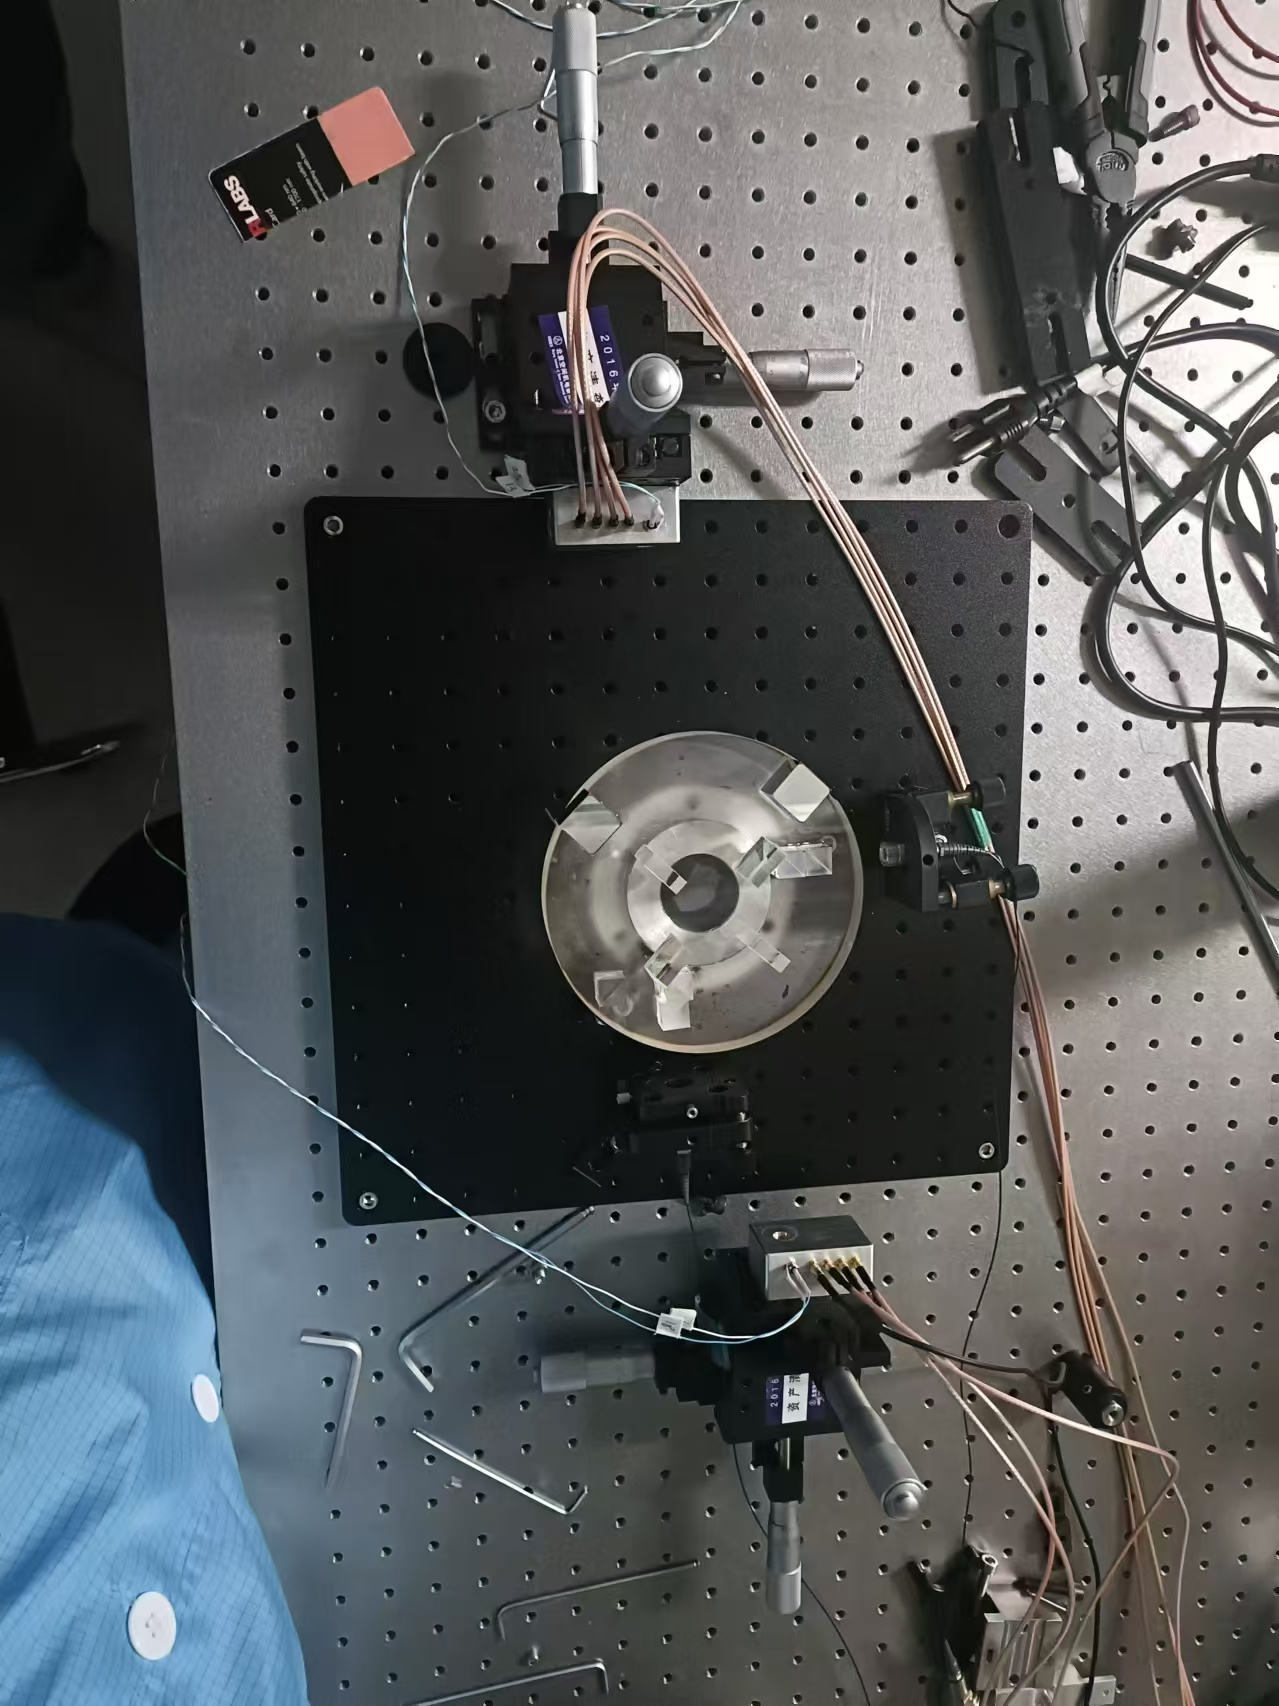
\includegraphics[width=\linewidth, height=0.45\textheight, keepaspectratio]{image/1.jpg}
        \vspace{0.5em} % 调整图片之间的间距
        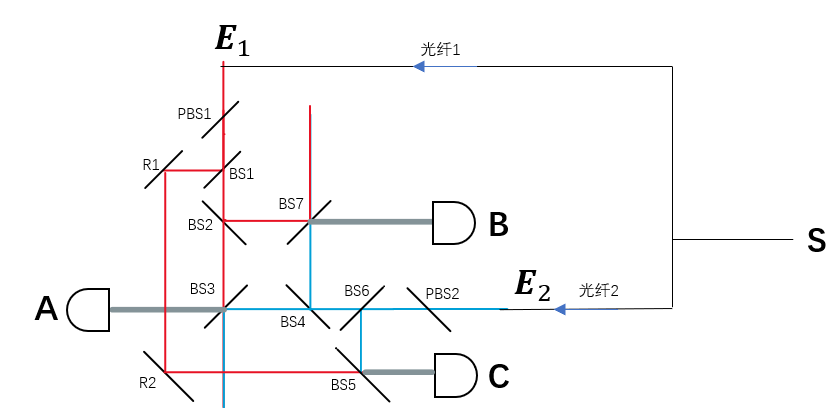
\includegraphics[width=\linewidth, height=0.45\textheight, keepaspectratio]{image/2.png}
    \end{minipage}
\end{frame}

\begin{frame}{干涉仪中的激光频率噪声}

    以探测器 $A$ 为例,设外差干涉的两束光均为平面波正入射。

    前面给出了探测器 $A$ 接收的功率为:

    $$
    \begin{aligned}
    P
    =P_{\mathrm{M}} + P_{\mathrm{R}} + 2\sqrt{P_{\mathrm{M}}P_{\mathrm{R}}}|o|\cos(\omega_{\mathrm{het}}t+\phi_{\mathrm{het}})
    \end{aligned}
    $$

    从光源 $S$ 经光纤 $1$ 到探测器 $A$ 的光程记为 $L_{A1}$

    从光源 $S$ 经光纤 $2$ 到探测器 $A$ 的光程记为 $L_{A2}$

    先不考虑光纤噪声,只考虑频率噪声,设 $t$ 时刻激光器产生的光场为:

    $$
    E(t)
    =E_0\cos[2\pi f_0 t+\phi_0(t)]
    $$

    则 $t$ 时刻在探测器 $A$ 的表面上干涉的两束光的相位差 $\phi_{\mathrm{het}} $ 为:
    
   $$
   \begin{aligned}
   \phi_{\mathrm{het}}
   =\phi_0\left(t-\frac{L_{A1}}{c}\right)-\phi_0\left(t-\frac{L_{A2}}{c}\right)
   \end{aligned}
   $$ 

   $\phi_{\mathrm{het}}$ 随时间的变化可以描述激光频率噪声。

   若 $L_{A1}=L_{A2}$,则 $\phi_{\mathrm{het}}=0$,此时激光频率噪声被消除。

\end{frame}

\section{光纤热噪声}
\begin{frame}{光纤热噪声}
    
    光纤热噪声是光纤传输中由于光纤材料的热扰动引起的噪声。

    环境热扰动 $\to$ 光纤长度扰动 $\to$ 光程扰动 $\to$ 相位扰动

    设光纤 $1,2$ 的光程的扰动分别为 $\delta L_1(t),\delta L_2(t)$,则相位扰动 $\delta \phi_{f1}(t),\delta \phi_{f2}(t) $ 分别为:

    $$
    \delta \phi_{f1}(t)
    =\frac{2\pi}{\lambda_0} \delta L_1(t),~~
    \delta \phi_{f2}(t)
    =\frac{2\pi}{\lambda_0} \delta L_2(t),~~
    $$

    不考虑频率噪声,只考虑光纤热噪声,探测器 $A$ 上的两束光的相位为:

    $$
    \phi_{\mathrm{M},A}
    =\phi_0-\frac{2\pi}{\lambda_0}L_{A1}+\delta \phi_{f1}(t)
    =\phi_0-\frac{2\pi}{\lambda_0}\left[L_{A1}-\delta L_1(t) \right]
    $$

    $$
    \phi_{\mathrm{R},A}
    =\phi_0-\frac{2\pi}{\lambda_0}L_{A2}+\delta \phi_{f2}(t)
    =\phi_0-\frac{2\pi}{\lambda_0}\left[L_{A2}-\delta L_2(t) \right]
    $$

    相位差为:

    $$
    \phi_{\mathrm{het},A}
    =\phi_{\mathrm{M},A}-\phi_{\mathrm{R},A}
    =-\frac{2\pi}{\lambda_0}\left[(L_{A1}-L_{A2}) + (\delta L_1(t)-\delta L_2(t)) \right]
    $$

\end{frame}

\begin{frame}
    探测器 $A$ 可作为参考干涉仪,其上的干涉信号不携带 test mass 的信息。
    
    对于携带 test mass 信息的探测器 $B$,其上的干涉信号的相位差还要多携带 test mass 的信息:

    $$
    \begin{aligned}
    \phi_{\mathrm{het},B}
    =-\frac{2\pi}{\lambda_0}\left[(L_{B1}-L_{B2}) + (\delta L_1(t)-\delta L_2(t)) \right] + \phi_{\mathrm{test}}
    \end{aligned}
    $$

    若能使光程满足 $L_{A1}-L_{A2}=L_{B1}-L_{B2} $,则可以得到:

    $$
    \phi_{\mathrm{test}}
    =\phi_{\mathrm{het},B}-\phi_{\mathrm{het},A}
    $$

\end{frame}

\section{实验}
\begin{frame}{实验光路}
    \begin{minipage}[t]{\textwidth}
        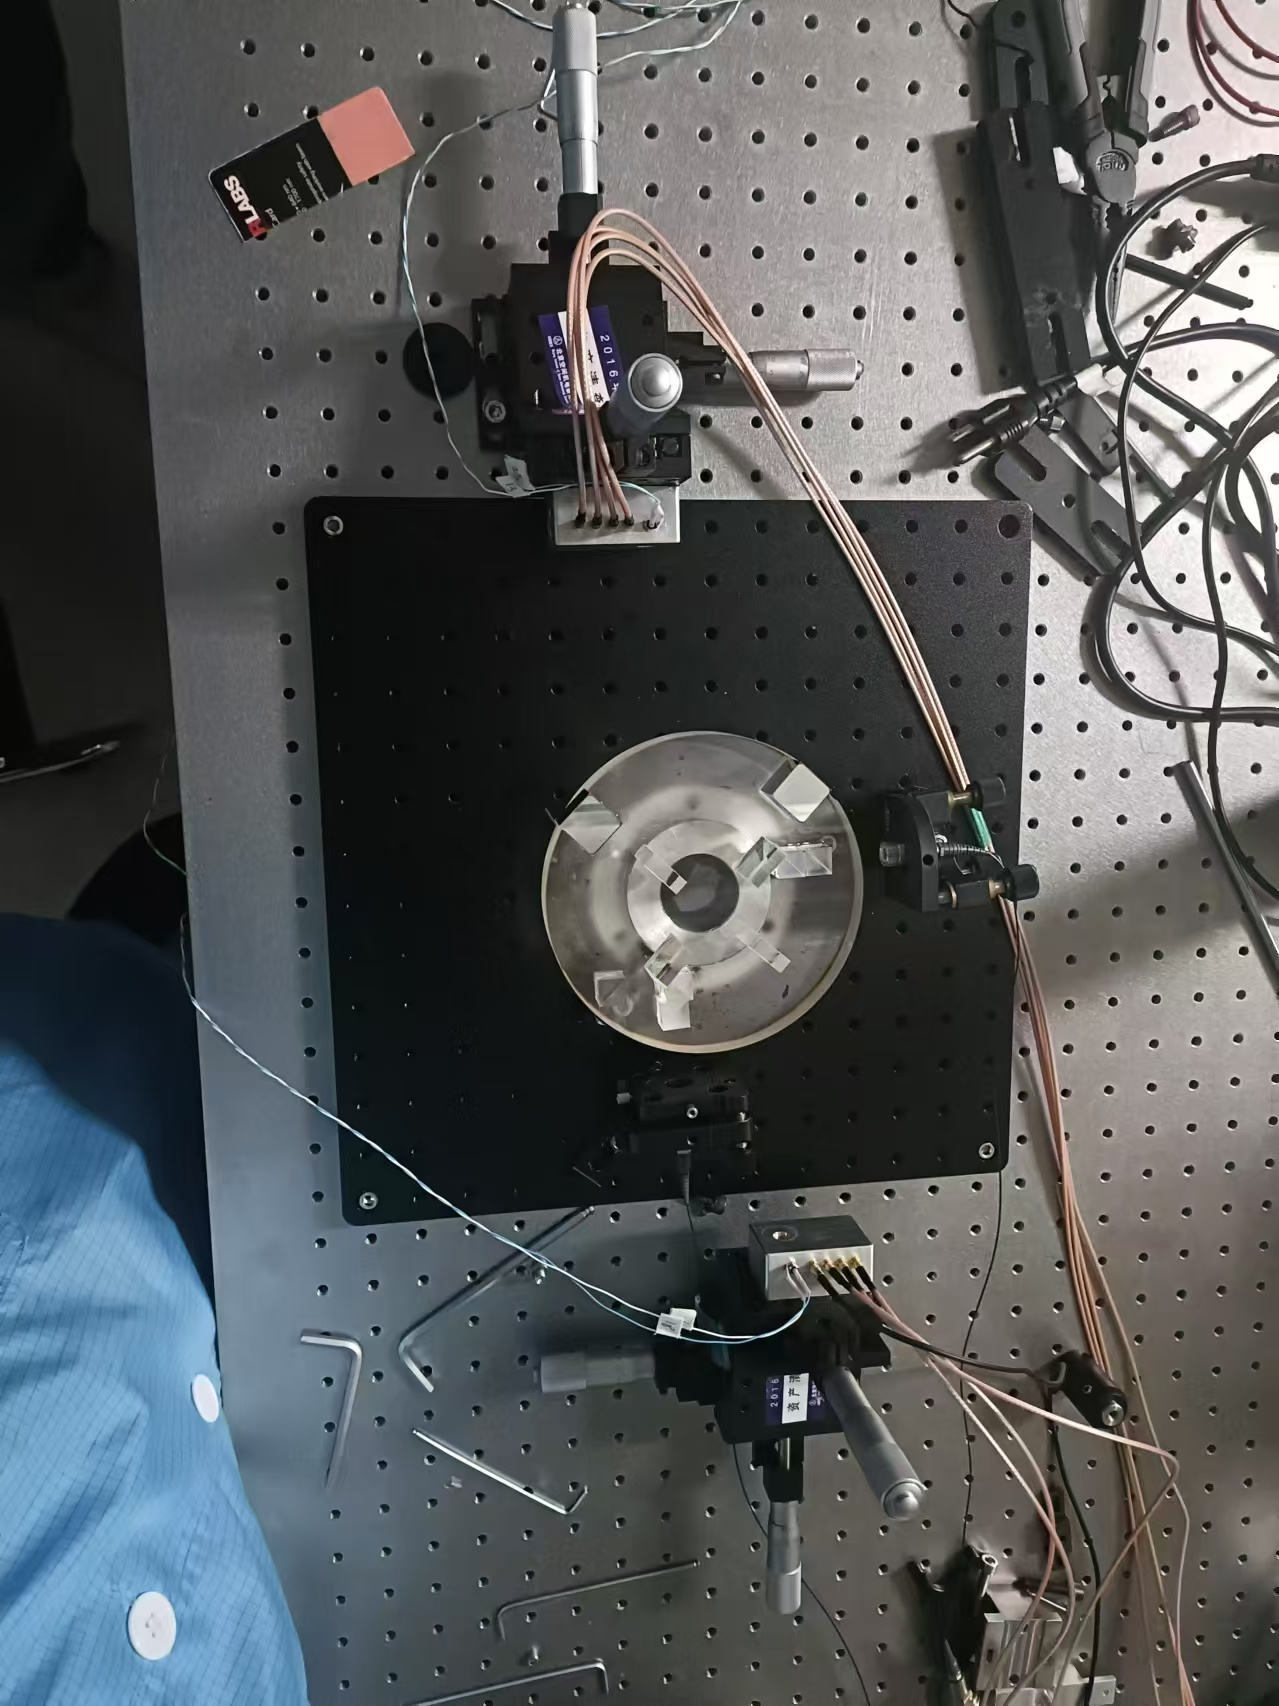
\includegraphics[width=\linewidth, height=0.45\textheight, keepaspectratio]{image/1.jpg}
        \vspace{0.5em} % 调整图片之间的间距
        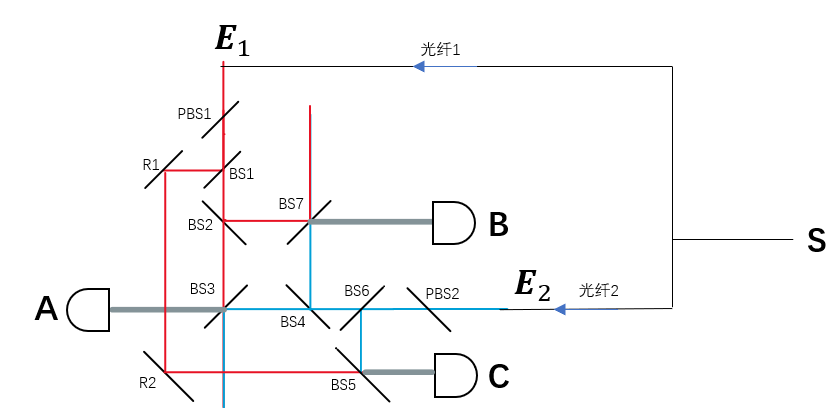
\includegraphics[width=\linewidth, height=0.45\textheight, keepaspectratio]{image/2.png}
    \end{minipage}
\end{frame}

\begin{frame}{数据}
    \begin{minipage}{0.5\textwidth}
        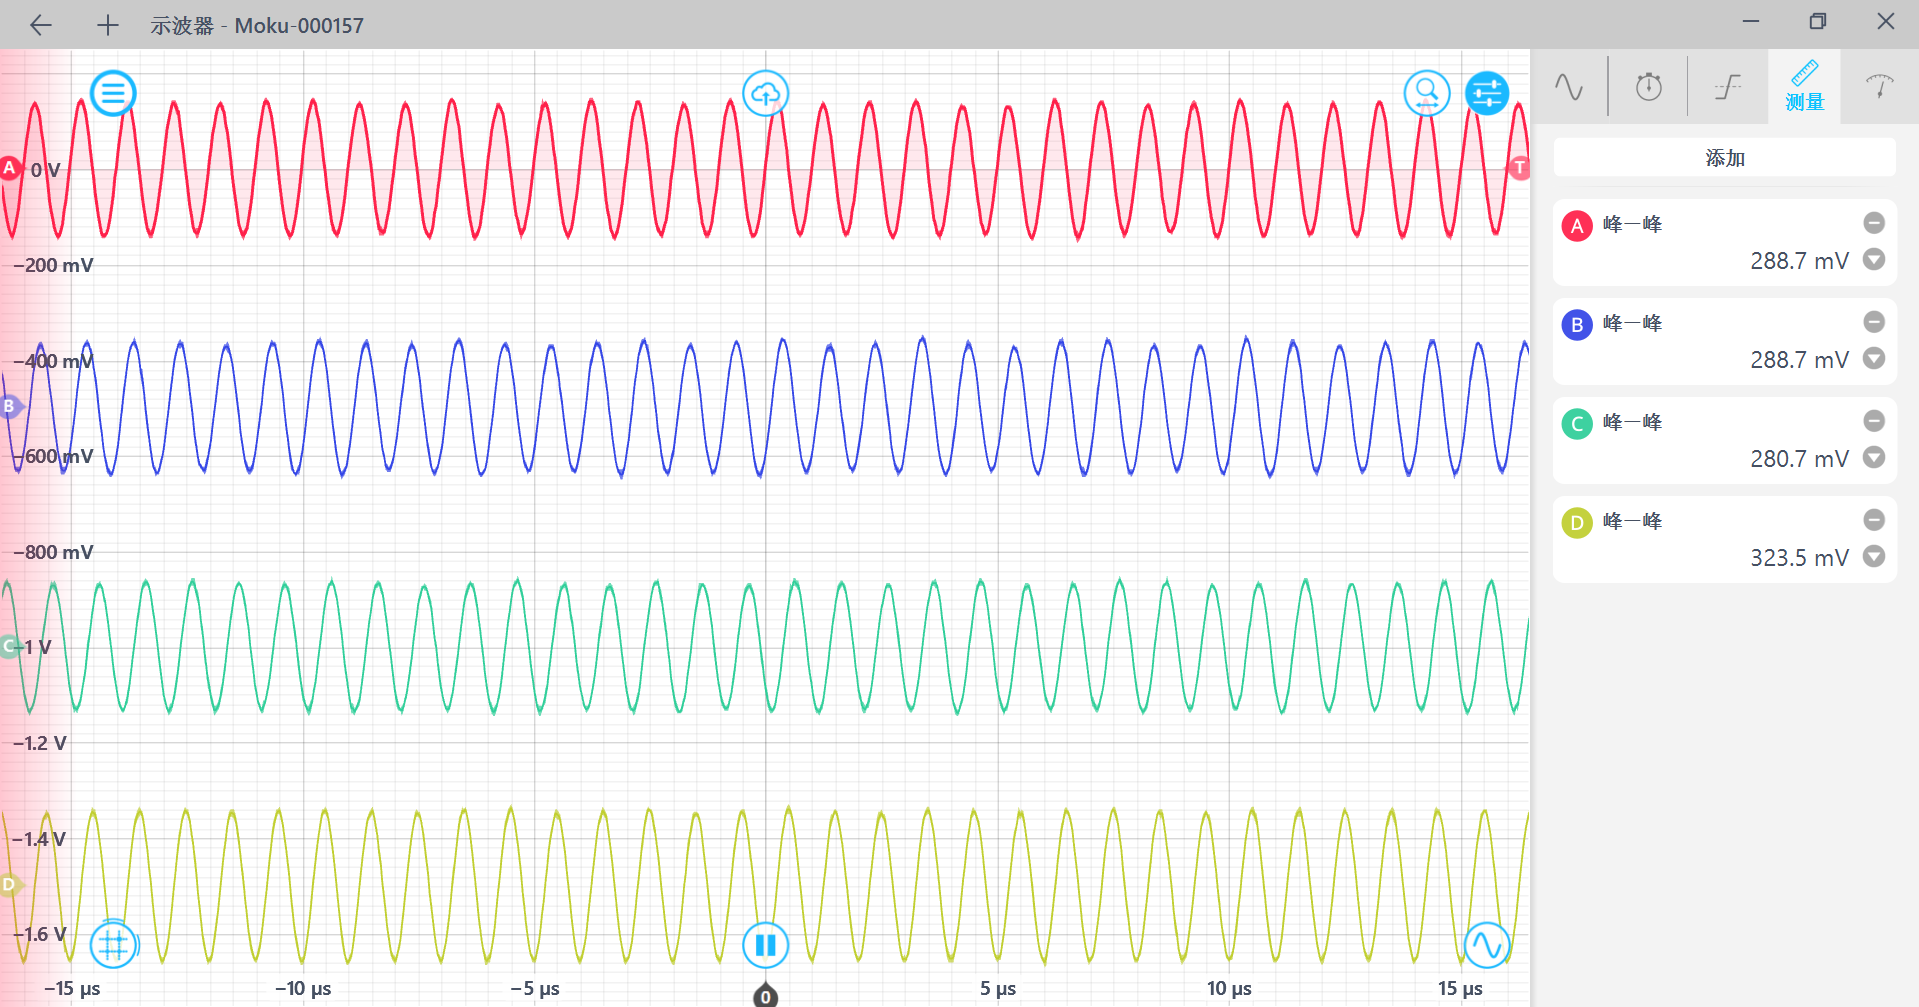
\includegraphics[width=\linewidth, height=0.45\textheight, keepaspectratio]{image/3.png}
        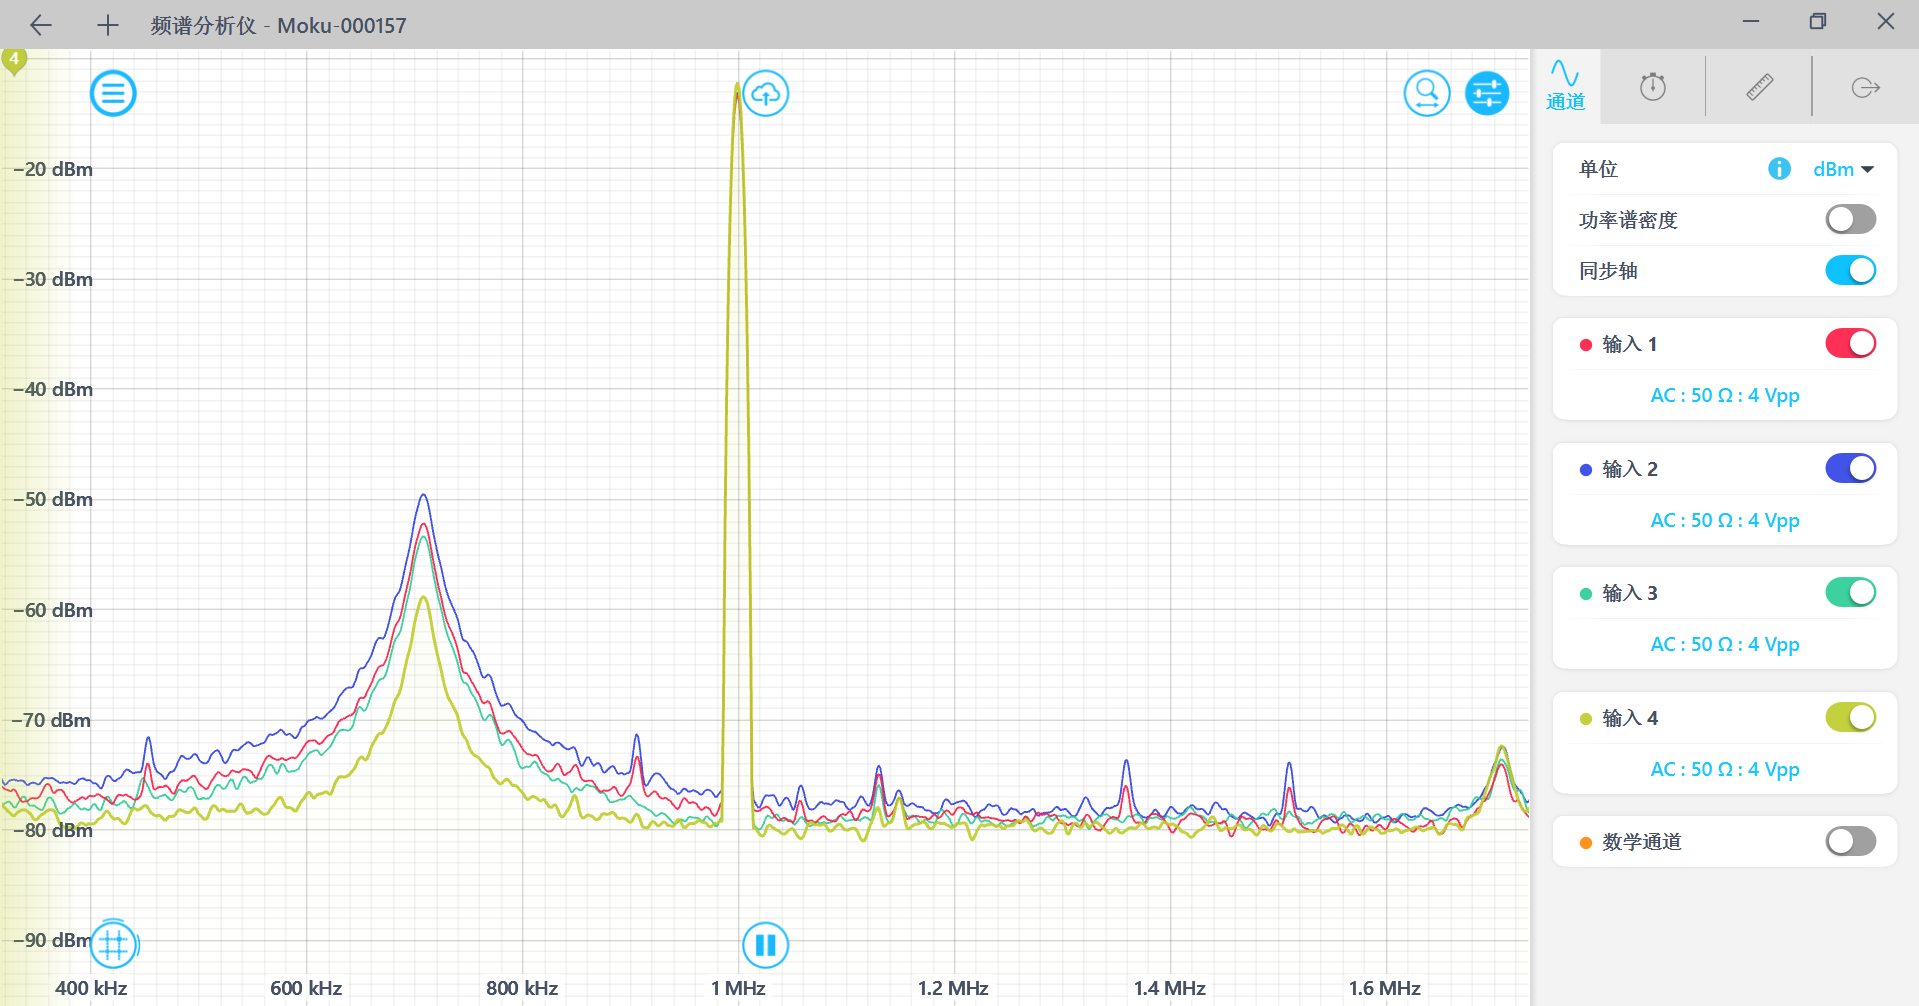
\includegraphics[width=\linewidth, height=0.45\textheight, keepaspectratio]{image/4.png}
    \end{minipage}%
    \begin{minipage}{0.5\textwidth}
        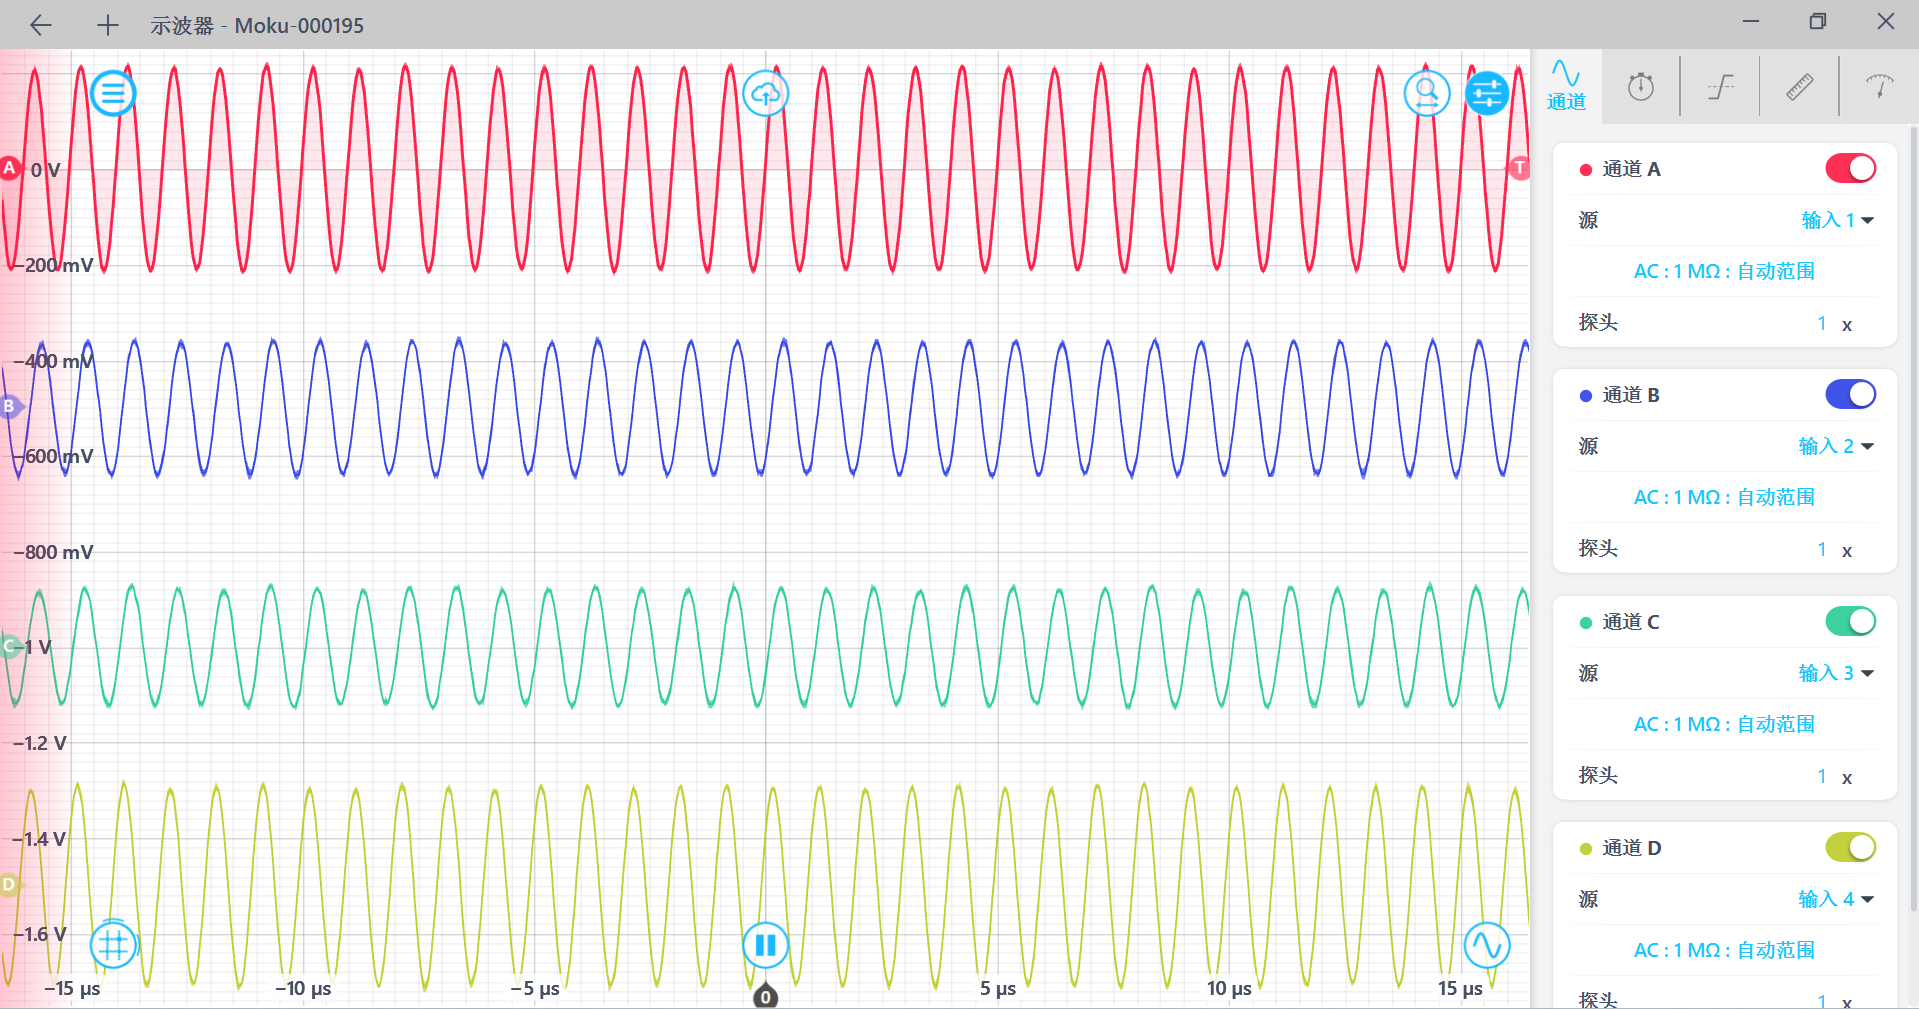
\includegraphics[width=\linewidth, height=0.45\textheight, keepaspectratio]{image/5.png}
        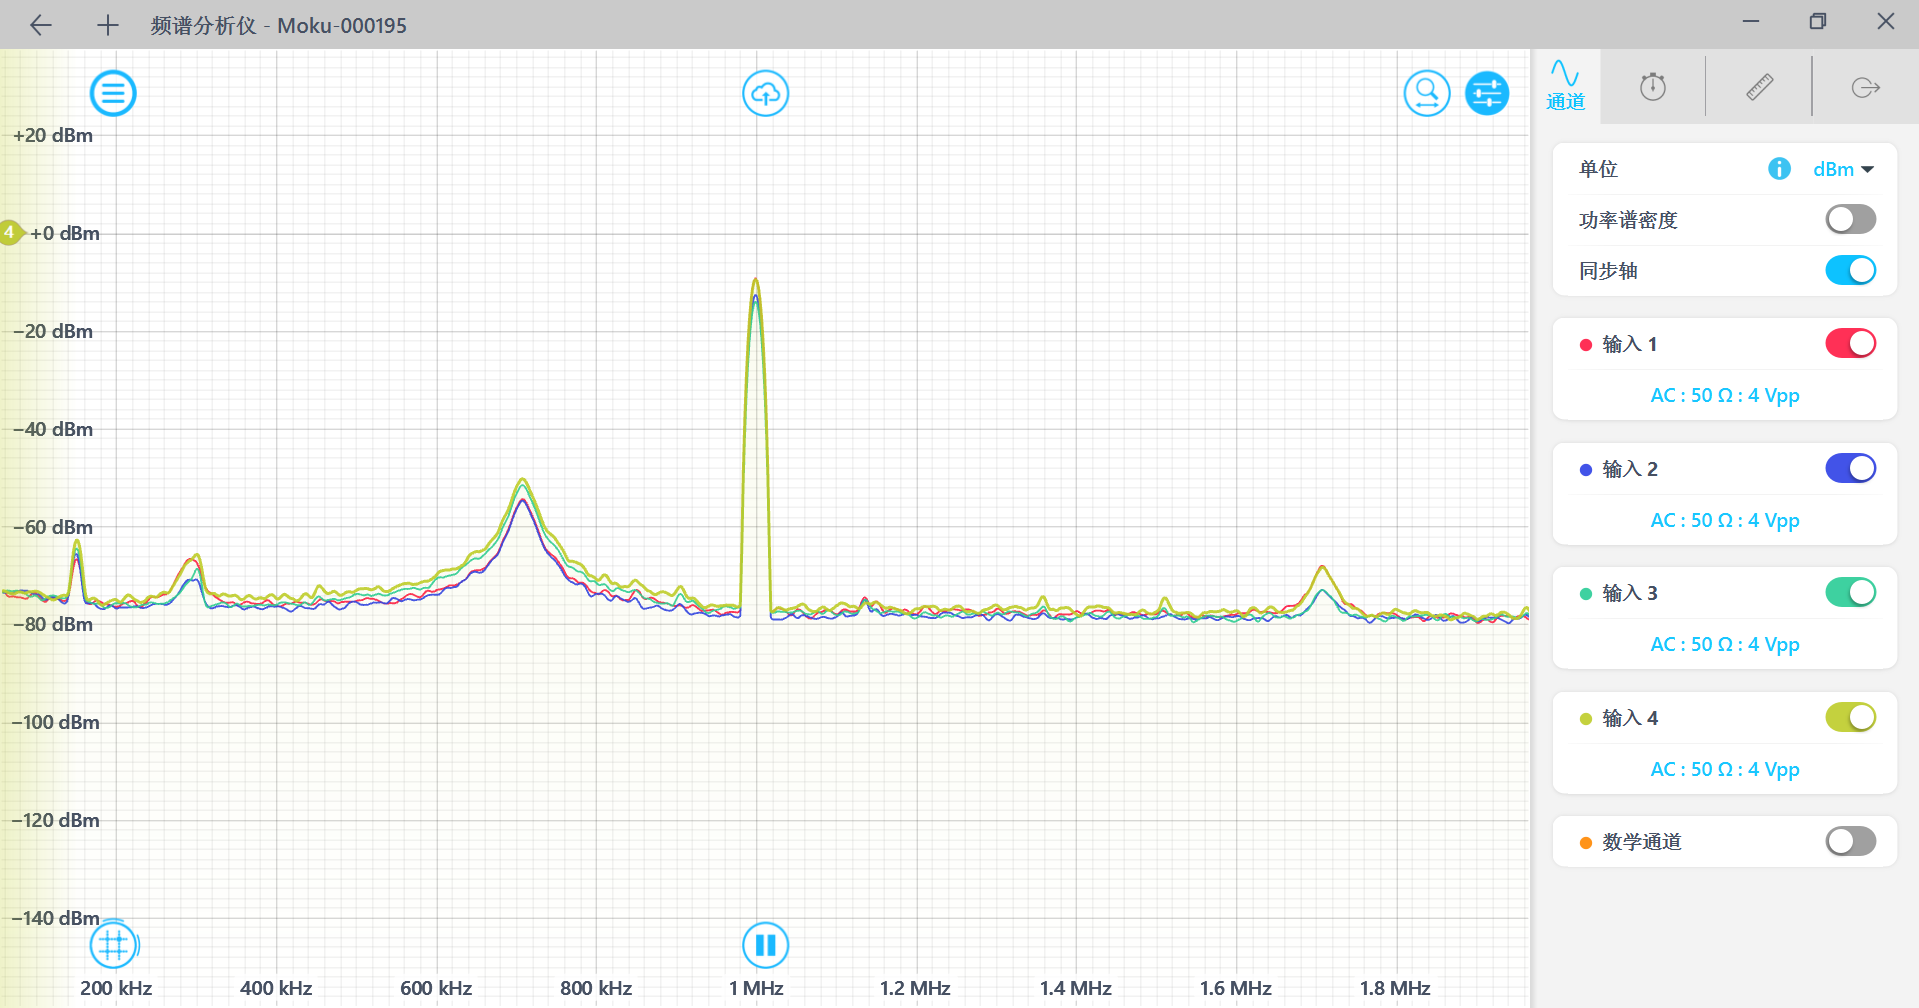
\includegraphics[width=\linewidth, height=0.45\textheight, keepaspectratio]{image/6.png}
    \end{minipage}
\end{frame}

\begin{frame}
    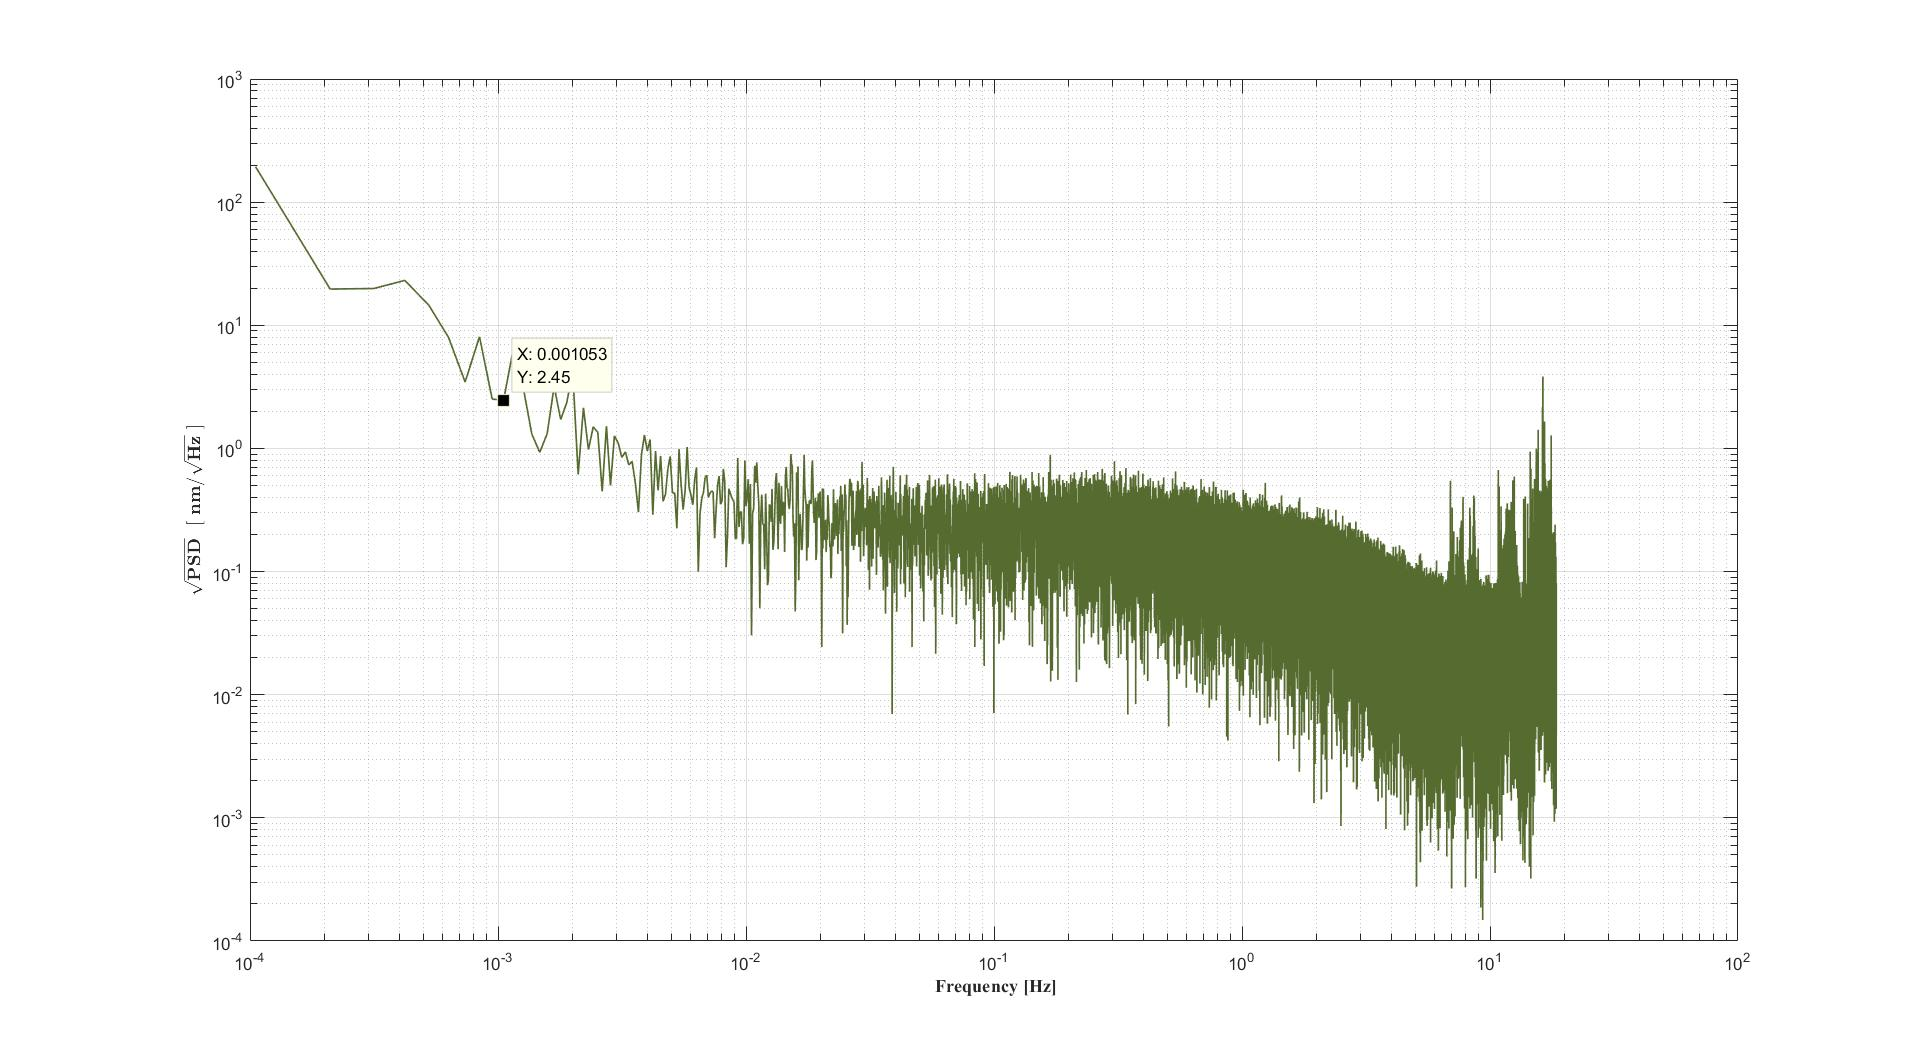
\includegraphics[width=\linewidth, height=0.65\textheight]{image/7.jpg}
    空气环境下静置的噪声功率谱密度,由探测器 $A,B$ 结果相减得到。
\end{frame}

\end{document}




